% Ad Lab II LaTeX template
% Dan Shields, Colorado School of Mines
% dshields@mymail.mines.edu
% 2017/01/01

% Developed for use by the students of Ad Lab II at Colorado School of Mines
% This program is not a final product and may contain errors

\documentclass[10pt,letterpaper]{journal}
\usepackage[margin=0.75in]{geometry}
\usepackage[tight,nice]{units}
\usepackage{graphicx,color,amsmath,amssymb}
\usepackage[numbers]{natbib}
\usepackage{url}
\usepackage{placeins}
\usepackage{float} % Place figures/tables exactly via capital H flag.
\usepackage{multirow}

\pagestyle{empty} % get rid of headers/footers by defalut.

\title{Advanced Lab II: Lab Template}
\subtitle{LAB \#?: A Lab}
\author{Dan Shields, Other Folks\\
  PH326 Section ? Lab Group ?\\
  Experiment Date: ...\\
  Report Due Date: ...}


\pagestyle{empty}

\begin{document}
\maketitle

\begin{abstract}

A NaI(Tl) scintillation detector was used in recording $\gamma$ emissions produced by $^{137}$Cs and $^{60}$Co. Other Things occurred. Some results were found with $\pm$ errors.

\end{abstract}

\begin{table*}
\begin{center}
\small{
\begin{tabular}[H]{|c|c|}\hline
Grade & \ \ \ Score \ \ \ \\\hline
Abstract and Cover Pg. & \\\hline
Fig. \& Plt. &  \\\hline
Data \& Error Ana. &  \\\hline
Writing &  \\\hline
Total &  \\\hline
\end{tabular}
}
\end{center}
\end{table*}


\pagebreak
%%%%%%%%%%%%%%%%%%%%%%%%%%%%%%%%%%%%%%%%%%%%%%%%%%%%%%%%%%%%%%%%%%%%%%%%%%%%%%%%
%%%%%%%%%%%%%%%%%%%%%%%%%%%%%%%%%%%%%%%%%%%%%%%%%%%%%%%%%%%%%%%%%%%%%%%%%%%%%%%%
\section{Introduction}
%%%%%%%%%%%%%%%%%%%%%%%%%%%%%%%%%%%%%%%%%%%%%%%%%%%%%%%%%%%%%%%%%%%%%%%%%%%%%%%%
%%%%%%%%%%%%%%%%%%%%%%%%%%%%%%%%%%%%%%%%%%%%%%%%%%%%%%%%%%%%%%%%%%%%%%%%%%%%%%%%
Some things were important to introduce the reader on about this lab.

%%%%%%%%%%%%%%%%%%%%%%%%%%%%%%%%%%%%%%%%%%%%%%%%%%%%%%%%%%%%%%%%%%%%%%%%%%%%%%%%
%%%%%%%%%%%%%%%%%%%%%%%%%%%%%%%%%%%%%%%%%%%%%%%%%%%%%%%%%%%%%%%%%%%%%%%%%%%%%%%%
\section{Apparatus}
%%%%%%%%%%%%%%%%%%%%%%%%%%%%%%%%%%%%%%%%%%%%%%%%%%%%%%%%%%%%%%%%%%%%%%%%%%%%%%%%
%%%%%%%%%%%%%%%%%%%%%%%%%%%%%%%%%%%%%%%%%%%%%%%%%%%%%%%%%%%%%%%%%%%%%%%%%%%%%%%%
 A cool figure (Figure \ref{fig:Scint}).

\begin{figure}[H]
  \begin{center}
    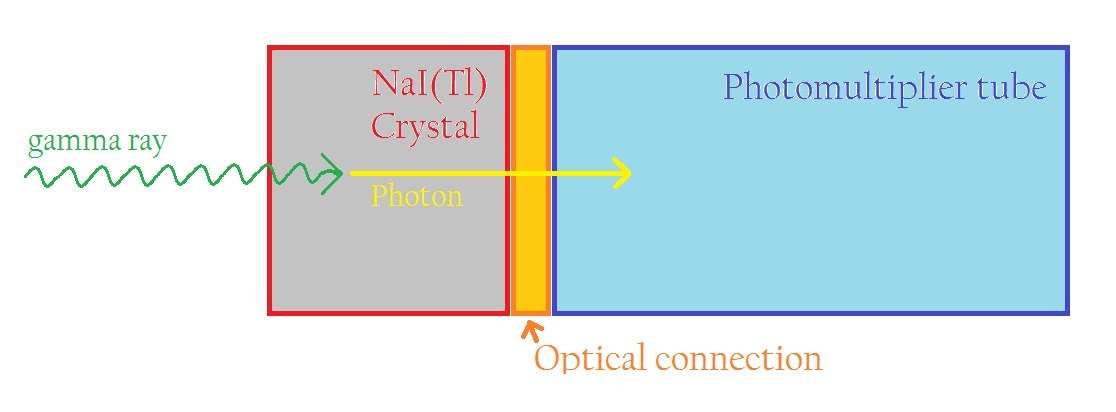
\includegraphics[width=8cm]{scintillator.jpg}
  \end{center}
  \caption{\scriptsize{NaI(Tl) detector, including the crystal, the optical coupling, and the photomultiplier tube.}}
  \label{fig:Scint}
\end{figure}

Yet another! (Figure \ref{fig:PMT}) This is getting interesting now. Really hooking the reader on your lab report.

\begin{figure}[H]
  \begin{center}
    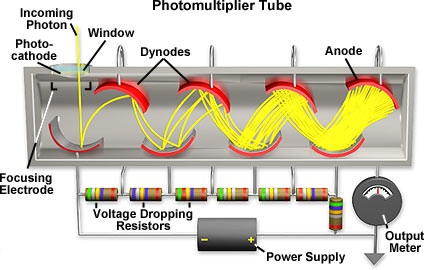
\includegraphics[width=8cm]{photomultiplier.jpg}
    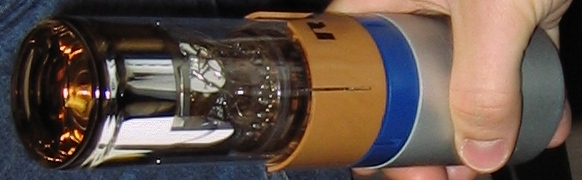
\includegraphics[width=8cm]{pm-base.jpg}
  \end{center}
  \caption{\scriptsize{Photomultiplier tube \cite{bib:PMT}. \label{fig:PMT}}}
\end{figure}

%%%%%%%%%%%%%%%%%%%%%%%%%%%%%%%%%%%%%%%%%%%%%%%%%%%%%%%%%%%%%%%%%%%%%%%%%%%%%%%%
%%%%%%%%%%%%%%%%%%%%%%%%%%%%%%%%%%%%%%%%%%%%%%%%%%%%%%%%%%%%%%%%%%%%%%%%%%%%%%%%
\section{Data Collection}
%%%%%%%%%%%%%%%%%%%%%%%%%%%%%%%%%%%%%%%%%%%%%%%%%%%%%%%%%%%%%%%%%%%%%%%%%%%%%%%%
%%%%%%%%%%%%%%%%%%%%%%%%%%%%%%%%%%%%%%%%%%%%%%%%%%%%%%%%%%%%%%%%%%%%%%%%%%%%%%%%

You might have used the MAESTRO\textsuperscript{\textregistered} software.

%%%%%%%%%%%%%%%%%%%%%%%%%%%%%%%%%%%%%%%%%%%%%%%%%%%%%%%%%%%%%%%%%%%%%%%%%%%%%%%%
%%%%%%%%%%%%%%%%%%%%%%%%%%%%%%%%%%%%%%%%%%%%%%%%%%%%%%%%%%%%%%%%%%%%%%%%%%%%%%%%
\section{Data Analysis}
%%%%%%%%%%%%%%%%%%%%%%%%%%%%%%%%%%%%%%%%%%%%%%%%%%%%%%%%%%%%%%%%%%%%%%%%%%%%%%%%
%%%%%%%%%%%%%%%%%%%%%%%%%%%%%%%%%%%%%%%%%%%%%%%%%%%%%%%%%%%%%%%%%%%%%%%%%%%%%%%%

Signals rise time was $\approx$20 $\unit{{\mu}s}$ and a fall time that is large comparatively at $\approx$300 $\unit{{\mu}s}$. Some data tables might look like:


\begin{table*}[h]
\begin{center}
\small{ 
\begin{tabular}{|c|c|c|c|c|c|}\hline
%\multicolumn{6}{|c|}{A nice title} \\\hline
Source                             & Energy (keV)        & Peak (bin)        & Fit FWHM (bin) & Net Area (bin) & Net Count Rate (s)  \\\hline
\tiny{$^{137}$Cs}                  &  661.657$\pm$0.0003 & 1$\pm$1   & 1 & 1$\pm$1 & 1 \\\hline
\multirow{2}{*}{\tiny{$^{60}$Co}}  & 1173.228$\pm$0.0003 & 1$\pm$1 & 1 &  1$\pm$1 & 1 \\\cline{2-6}
                                   & 1332.492$\pm$0.0004 & 1$\pm$1 & 1 &  1$\pm$1 & 1 \\\hline
\tiny{$^{40}$K}                    & 1460.822$\pm$0.0006 & 1$\pm$1 &  1 &      1$\pm$1 & 1 \\\hline
\end{tabular}
}
\caption{Spectral information from MAESTRO\textsuperscript{\textregistered}. Energy from \cite{bib:nuclear}}
\end{center}
\end{table*}

A fancy equation:

\begin{equation}
 Energy= m x + B
\end{equation}


You probably will use \cite{bib:error} to do some error analysis.

\begin{figure}[H]
\begin{center}
  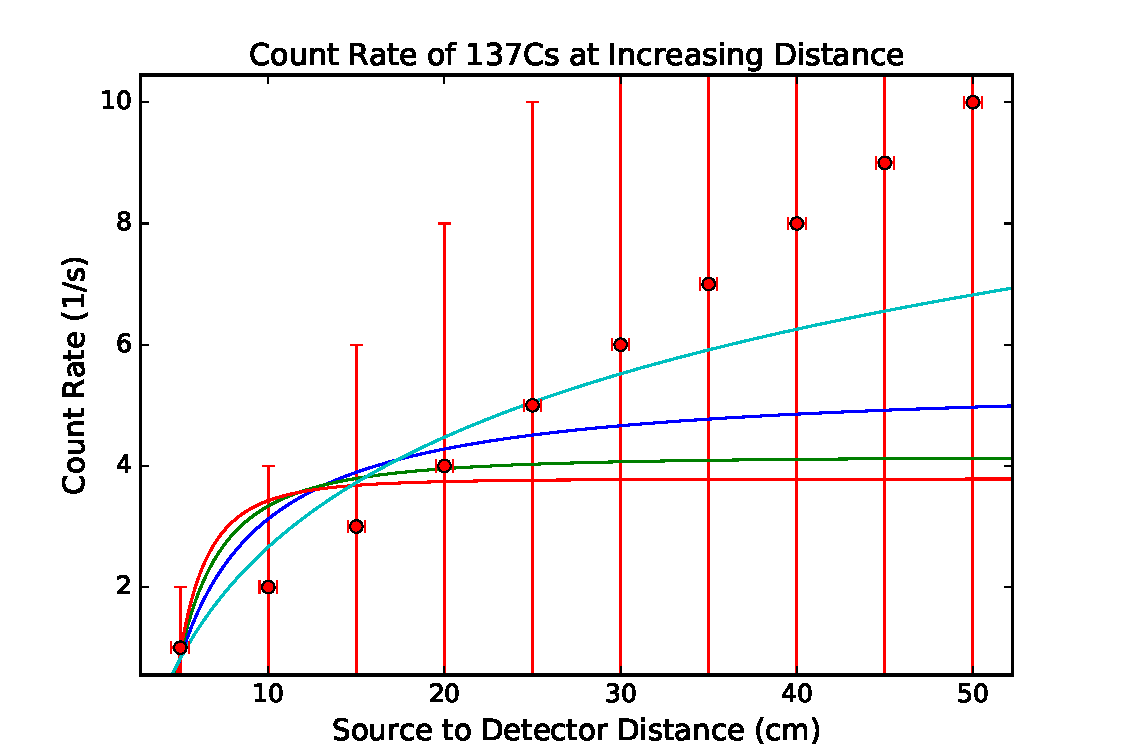
\includegraphics[width=3in]{dist_fit.pdf}                                              
\end{center}  
\caption{$r^{-1}$=Blue,$r^{-2}$=Green, $r^{-3}$=Red, $r^{-?}$ , Data=Blue points}                                      
\end{figure}

%%%%%%%%%%%%%%%%%%%%%%%%%%%%%%%%%%%%%%%%%%%%%%%%%%%%%%%%%%%%%%%%%%%%%%%%%%%%%%%%
%%%%%%%%%%%%%%%%%%%%%%%%%%%%%%%%%%%%%%%%%%%%%%%%%%%%%%%%%%%%%%%%%%%%%%%%%%%%%%%%
\section{Conclusion}
%%%%%%%%%%%%%%%%%%%%%%%%%%%%%%%%%%%%%%%%%%%%%%%%%%%%%%%%%%%%%%%%%%%%%%%%%%%%%%%%
%%%%%%%%%%%%%%%%%%%%%%%%%%%%%%%%%%%%%%%%%%%%%%%%%%%%%%%%%%%%%%%%%%%%%%%%%%%%%%%%
Some good and bad things happened.

\newpage
\begin{thebibliography}{99}

  \bibitem{bib:LW} Lawrence Wiencke, Professor for PHGN-326.  Instructions for Experiments: Experiment 1: Scintillation Detector. Colorado School of Mines, Physics Department, 2017.  
  \bibitem{bib:PMT} Mortimer Abramowitz \& Michael W. Davidson, ``Concepts in Digital Imaging Technology, Photomultiplier Tubes'', Last modification: Friday, Jul 16, 2004 at 08:16 AM, \url{http://micro.magnet.fsu.edu/primer/digitalimaging/concepts/photomultipliers.html}
	\bibitem{bib:2} C.R. Nave, ``Inverse Square Law, Radiation'', Georgia State University, Department of Physics and Astronomy, 2006, \url{http://hyperphysics.phy-astr.gsu.edu/HBASE/forces/isq.html}
  \bibitem{bib:error} John R. Taylor, Professor at the University of Colorado Department of Physics.``An Introduction to Error Analysis: The Study of Uncertainties in Physical Measurements'' Second Edition, 1982.
  \bibitem{bib:nuclear} S.Y.F. Chu, L.P. Ekström, and R.B. Firestone1. ``The Lund/LBNL Nuclear Data Search'', Last Modification:February 1999, \url{http://nucleardata.nuclear.lu.se/nucleardata/toi/perchart.htm}
\end{thebibliography}

\end{document}
